\usetikzlibrary{calc}
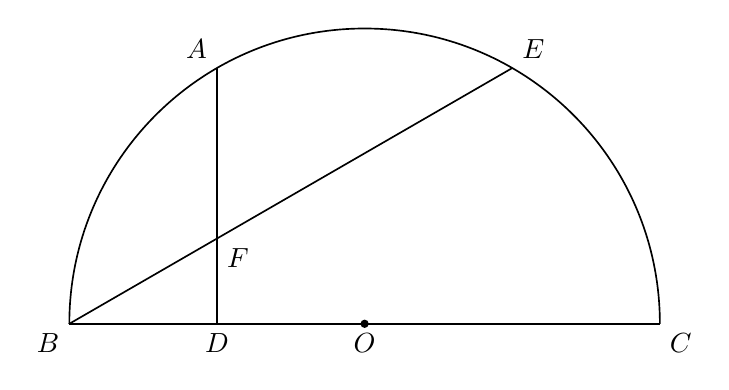
\begin{tikzpicture}[x=1cm,y=1cm,line width=.6pt,font=\normalsize]
\coordinate (O) at (0,0);
\coordinate (B) at (-3.75,0);
\coordinate (C) at (3.75,0);
\coordinate (A) at (-1.875,3.2476);
\coordinate (E) at (1.875,3.2476);
\coordinate (D) at (-1.875,0);
\coordinate (F) at (-1.875,1.08253);
\draw (B) arc[start angle=180,end angle=0,radius=3.75cm];
\draw (B)--(C);
\draw (A)--(D);
\draw (B)--(E);
\fill (O) circle (1.5pt);
\node[below left] at (B) {$B$};
\node[below] at (D) {$D$};
\node[below] at (O) {$O$};
\node[below right] at (C) {$C$};
\node[above left] at (A) {$A$};
\node[above right] at (E) {$E$};
\node[below right] at (F) {$F$};
\end{tikzpicture}
